
\section{Results}

\subsection{TD-Error Magnitude Is Not a Universal Progress Signal}

We first test the premise underlying TD-error-driven adaptive exploration: that the magnitude of the temporal-difference error should decrease as learning progresses. Figure~\ref{fig:td-diagnostic} compares the evolution of mean absolute TD error with greedy evaluation performance under both linear Sarsa($\lambda$) and tuned Double DQN.

The results do not support a universal monotonic relationship. Under linear function approximation, the TD-error change from the early to late training region is \LinearMountainCarTDChangePct\% on MountainCar, \LinearCartPoleTDChangePct\% on CartPole, \LinearAcrobotTDChangePct\% on Acrobot, and \LinearLunarLanderTDChangePct\% on LunarLander. In particular, CartPole improves substantially while the TD-error magnitude increases rather than decreases. The same phenomenon is present under nonlinear approximation: the corresponding changes under Double DQN are \DQNMountainCarTDChangePct\%, \DQNCartPoleTDChangePct\%, \DQNAcrobotTDChangePct\%, and \DQNLunarLanderTDChangePct\%.

These results do not imply that TD error is uninformative. Rather, they show that its absolute magnitude is not a universal monotone proxy for learning progress under function approximation. Consequently, an exploration rule that interprets a large raw TD error as evidence that additional exploration is necessarily required can receive a qualitatively misleading signal late in training.

\begin{figure}[t]
    \centering
    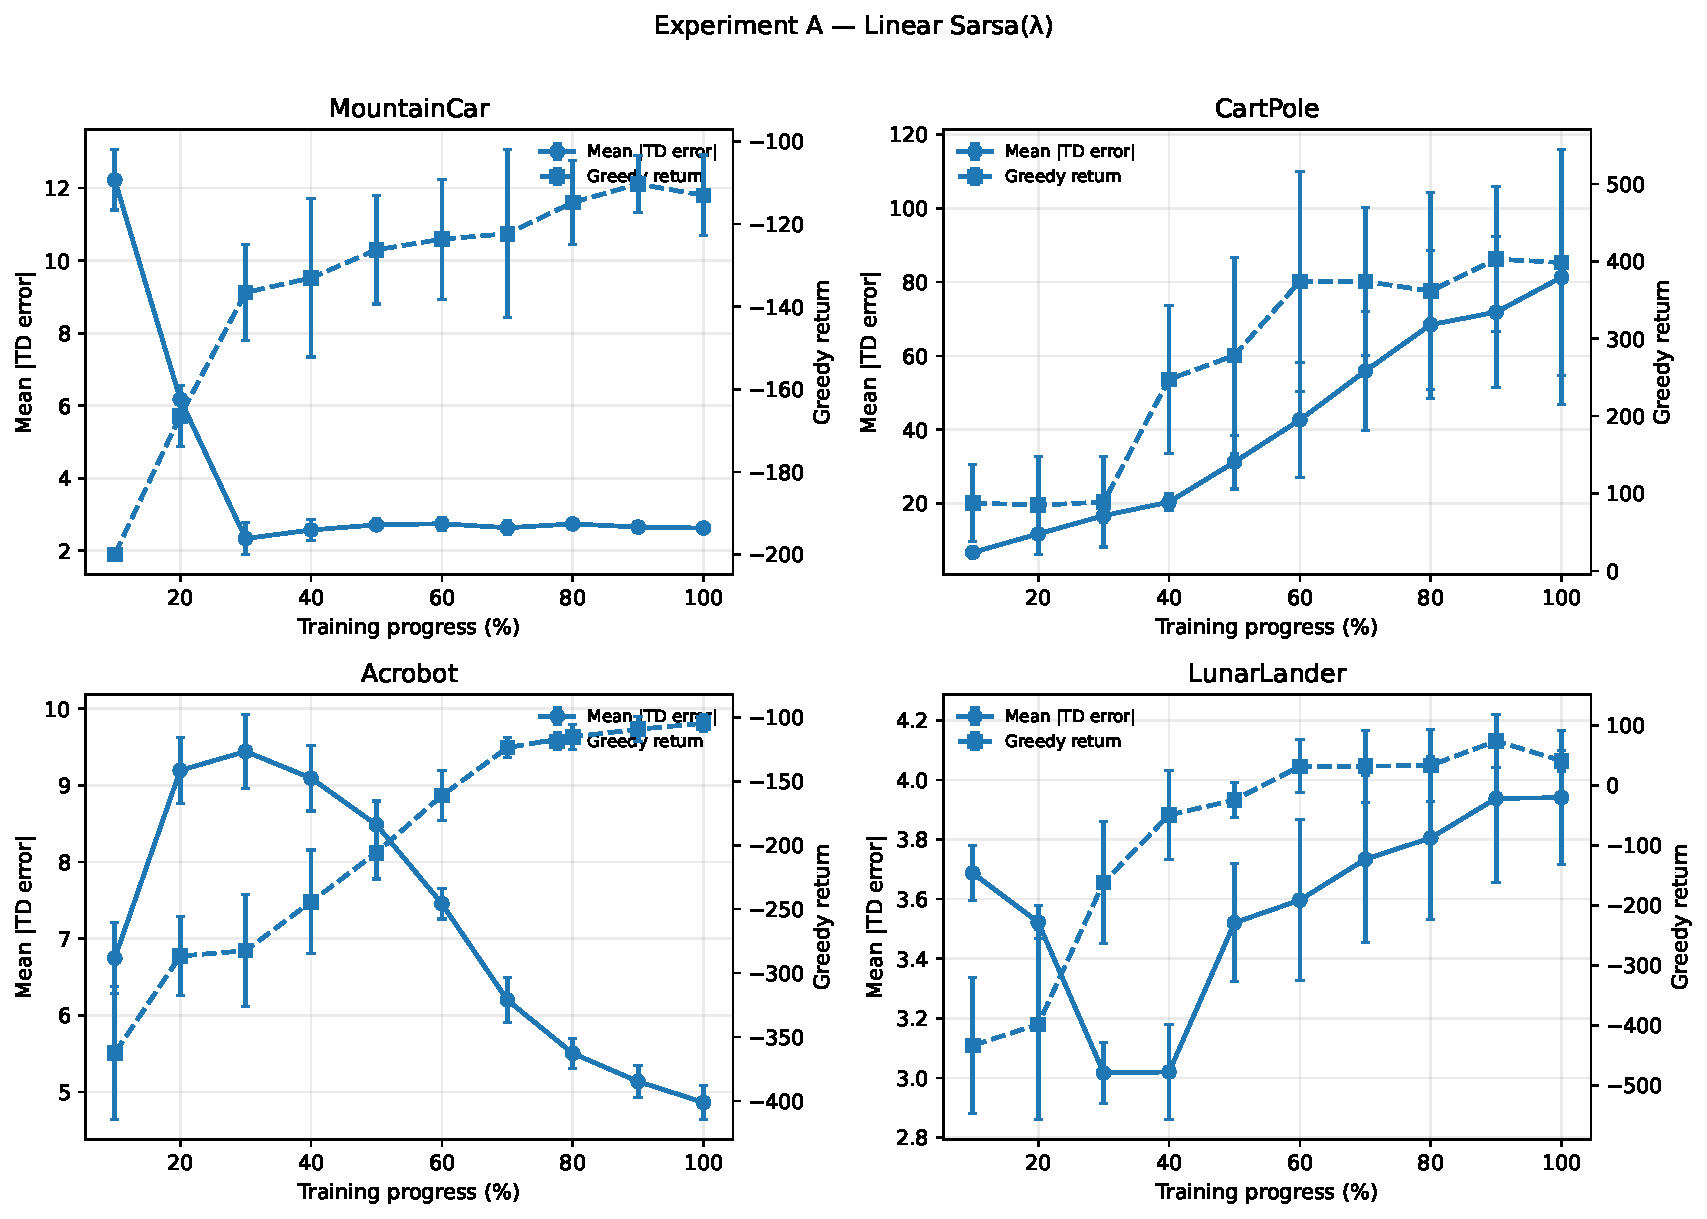
\includegraphics[width=\columnwidth]{src/figures/final/diagnostics/diag_A_td_error_linear.pdf}
    \caption{Evolution of mean absolute TD error and greedy evaluation return under linear Sarsa($\lambda$). The relationship between TD-error magnitude and policy improvement is environment dependent.}
    \label{fig:td-linear}
\end{figure}

\begin{figure}[t]
    \centering
    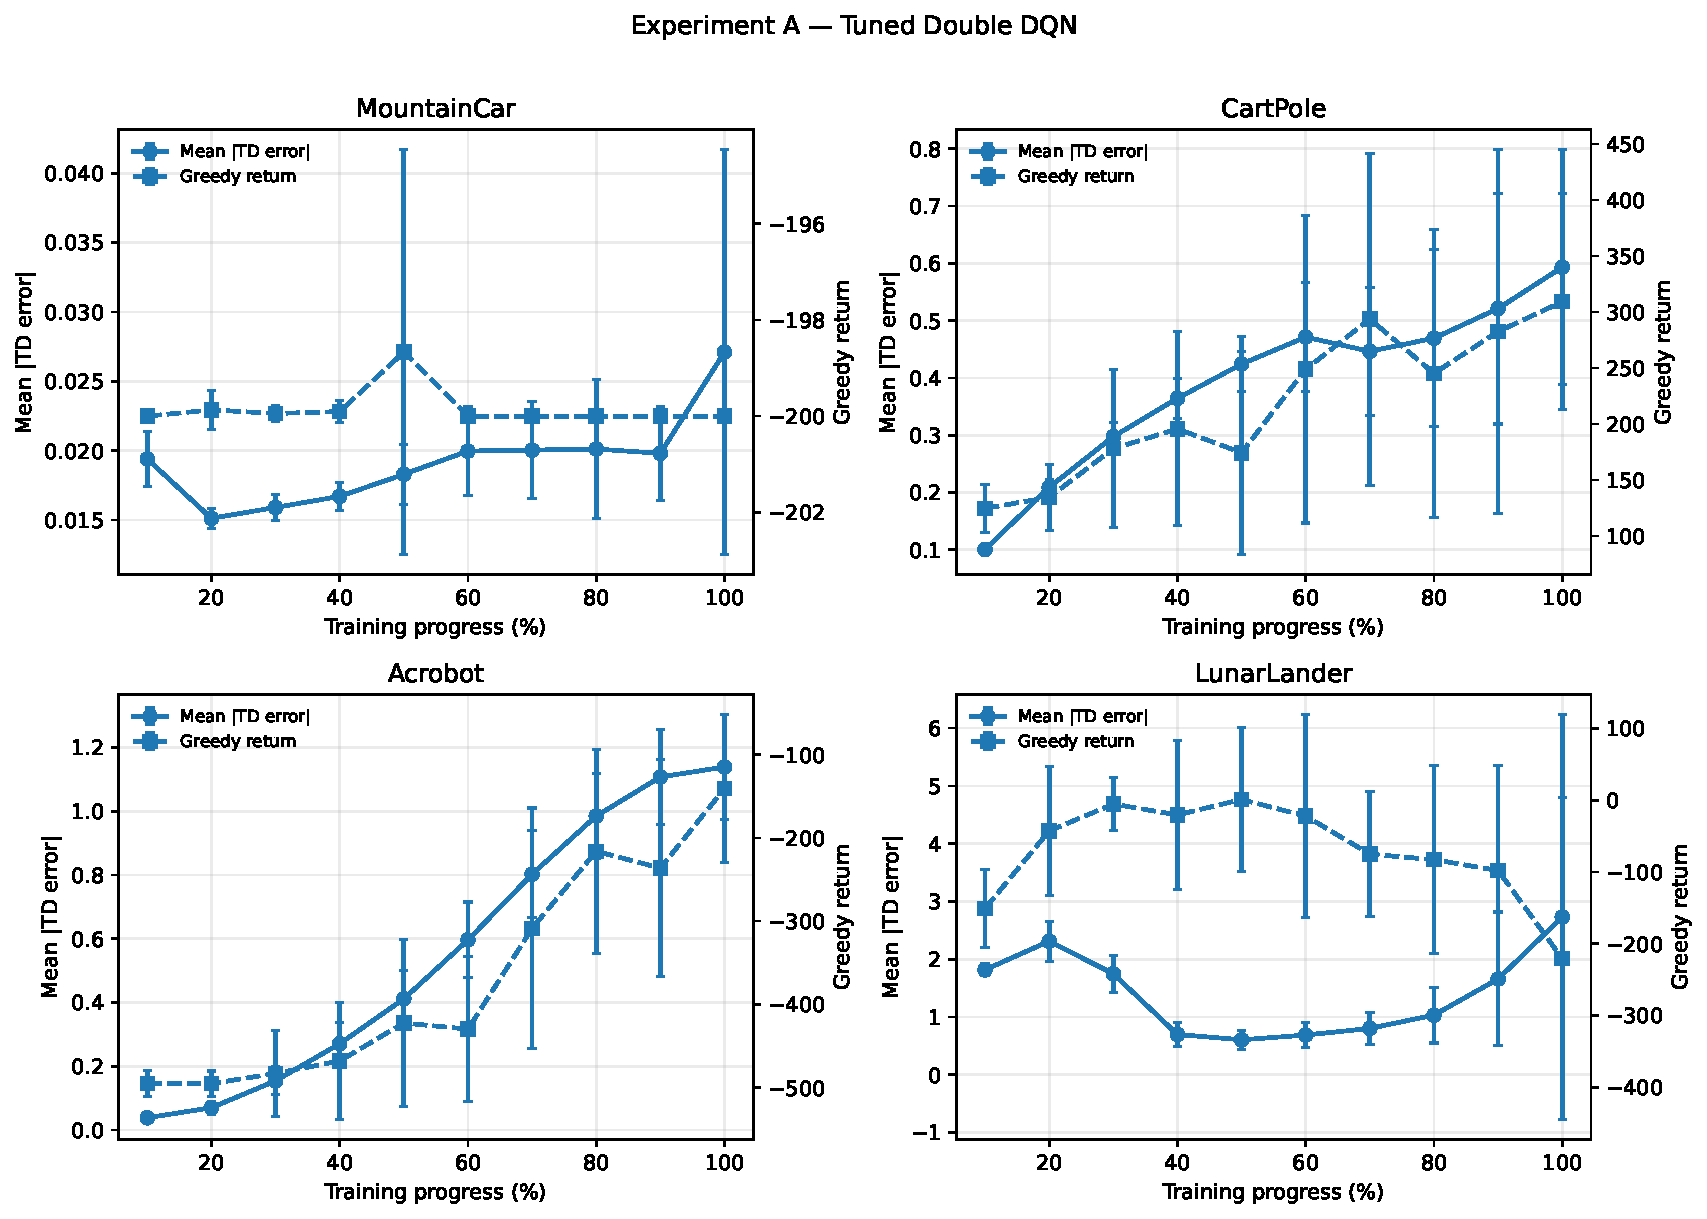
\includegraphics[width=\columnwidth]{src/figures/final/diagnostics/diag_A_td_error_dqn.pdf}
    \caption{TD-error diagnostic under tuned Double DQN. Increasing or persistently large TD errors can coexist with improving control performance.}
    \label{fig:td-diagnostic}
\end{figure}


\subsection{VDBE Approaches a TD-Independent Limit}

We next isolate the dependence of VDBE on its scale parameter $\sigma$. The VDBE update depends on the normalized magnitude $|\delta|/\sigma$. Therefore, as $\sigma$ becomes very large, this ratio approaches zero and the influence of the TD-error magnitude on the exploration update vanishes.

Figure~\ref{fig:vdbe-limit} evaluates this transition explicitly on MountainCar and Acrobot under both function approximators. Large finite values of $\sigma$ converge empirically toward the separately implemented $\sigma=\infty$ condition. The exact-convergence diagnostic further shows that, at sufficiently large finite $\sigma$, stored evaluation behavior becomes indistinguishable from the explicit TD-independent limit.

This establishes the limiting behavior empirically, but it does not show that the limit is desirable. In both tested environments under linear approximation, and likewise in the Double-DQN diagnostic, the highest mean return is obtained at a finite value of $\sigma$ rather than at the TD-independent limit. Thus, the experiment identifies a degeneration mechanism without claiming that VDBE is best when its adaptive signal disappears.

\begin{figure}[t]
    \centering
    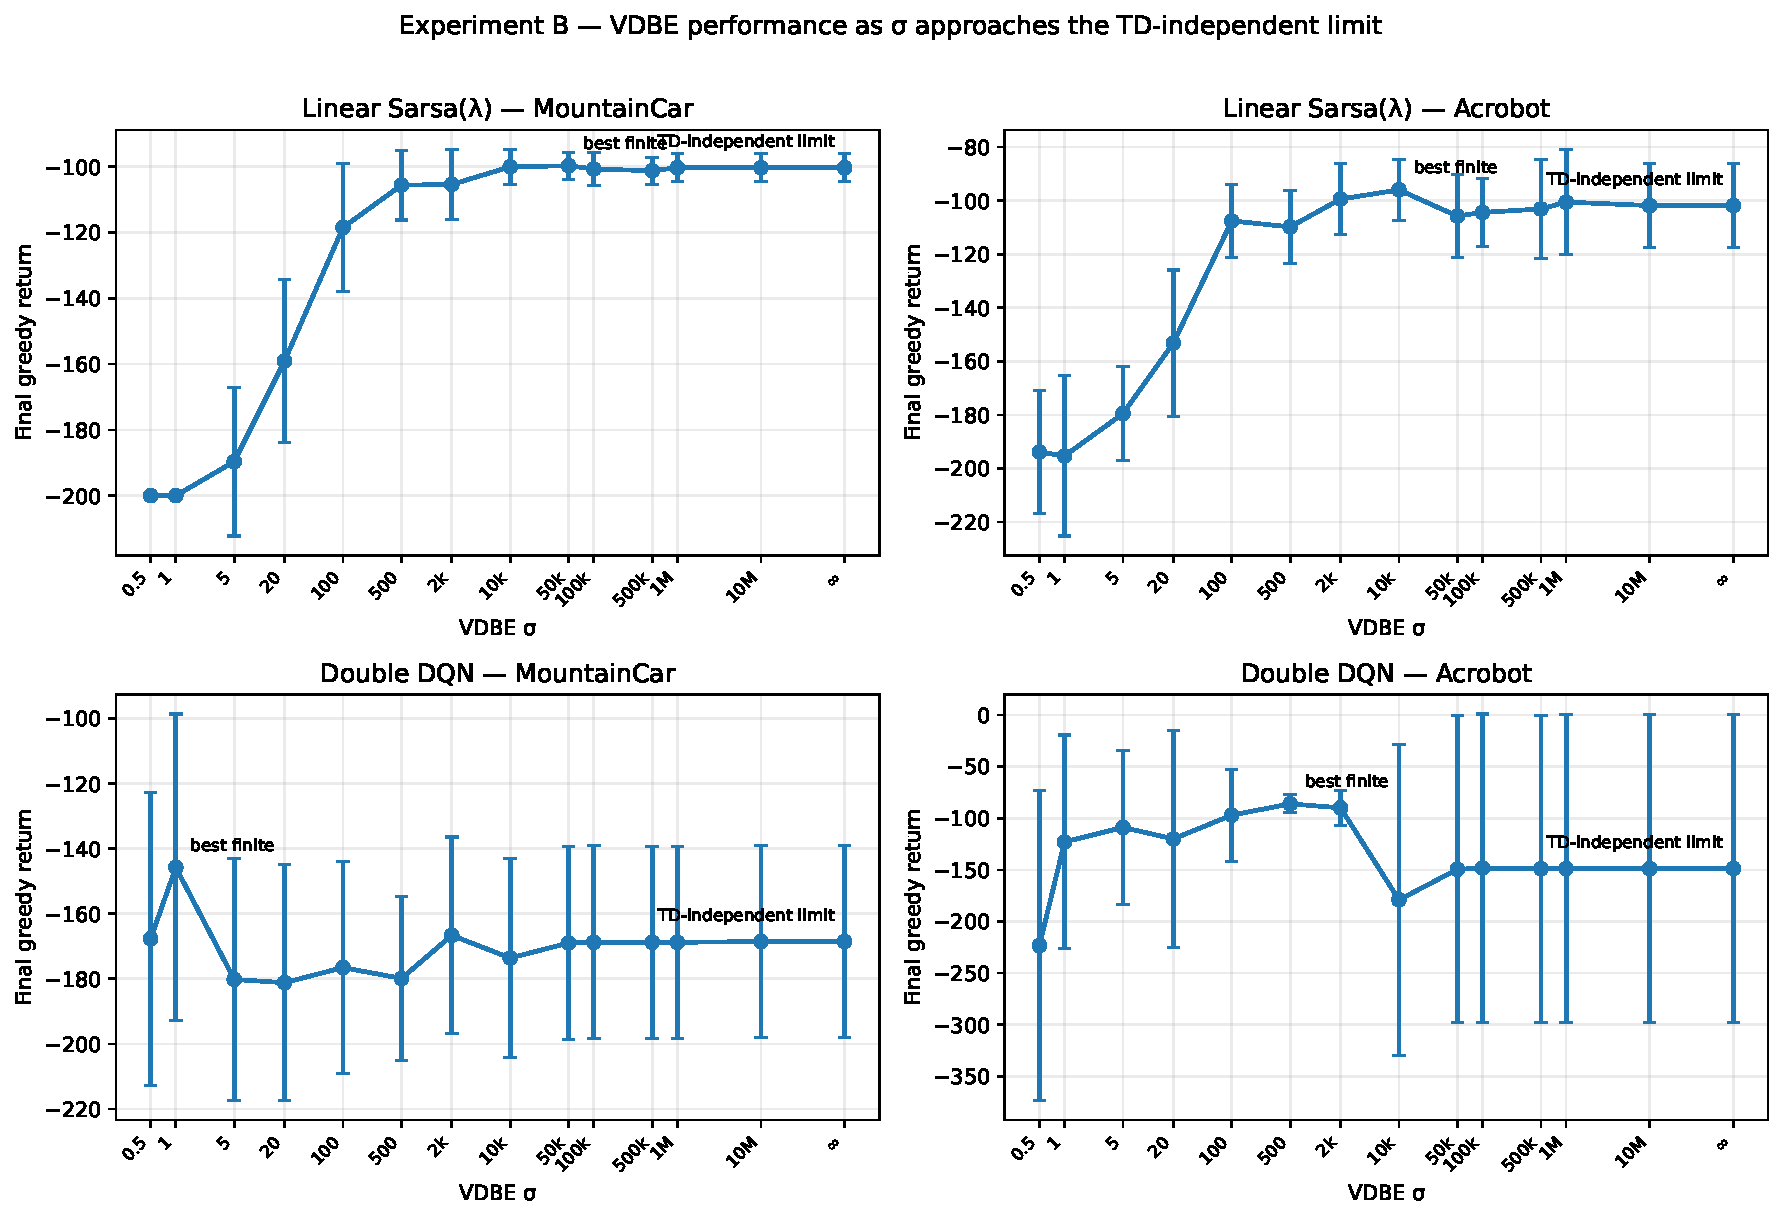
\includegraphics[width=\columnwidth]{src/figures/final/diagnostics/diag_B_vdbe_limit_performance.pdf}
    \caption{VDBE performance as $\sigma$ increases toward the TD-independent limit. The explicit infinite-$\sigma$ condition is shown together with finite settings.}
    \label{fig:vdbe-limit}
\end{figure}

\begin{figure}[t]
    \centering
    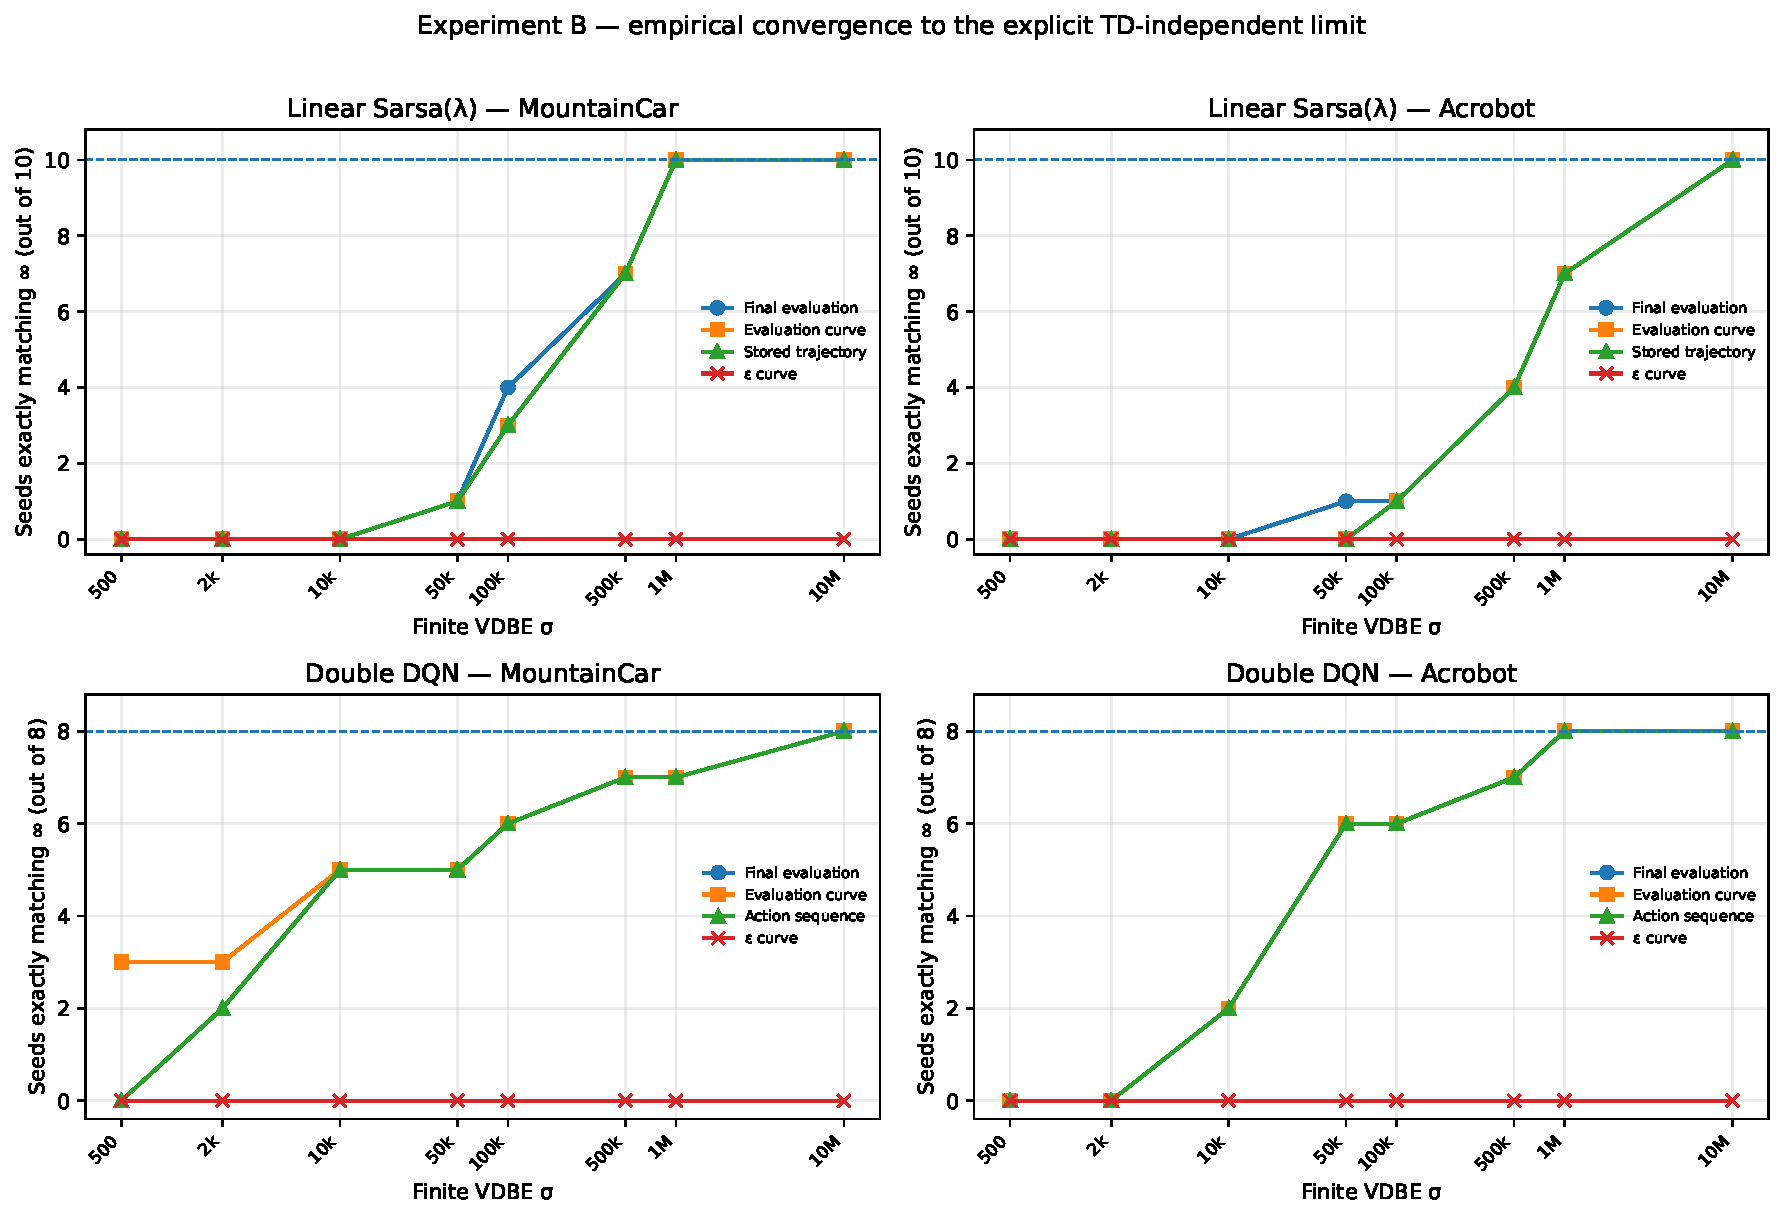
\includegraphics[width=\columnwidth]{src/figures/final/diagnostics/diag_B_vdbe_exact_convergence.pdf}
    \caption{Number of seeds for which large finite-$\sigma$ VDBE exactly matches the explicit TD-independent limit on stored diagnostics.}
    \label{fig:vdbe-exact}
\end{figure}


\subsection{RATE Removes Positive Reward-Scale Dependence}

RATE replaces an absolute TD-error signal with the dimensionless ratio
\begin{equation}
    \rho_t =
    \frac{m_{\delta,t}}
    {m_{\delta,t}+m_{v,t}},
\end{equation}
where $m_{\delta,t}$ and $m_{v,t}$ are exponential moving averages of $|\delta_t|$ and the magnitude of the corresponding value estimate. Under a positive reward rescaling by a constant $c$, the ideal linear value estimates and TD errors scale by the same factor. Consequently, both terms of the ratio scale together and $c$ cancels.

The controlled reward-scale experiment confirms this behavior under linear function approximation. Across reward multipliers $c\in\{0.01,1,100\}$, the spread in mean final greedy evaluation is \RateRewardScaleSpread\ points for RATE and \DecayRewardScaleSpread\ points for the reward-independent decay control, compared with \VdbeRewardScaleSpread\ points for fixed-$\sigma$ VDBE. Figure~\ref{fig:reward-scale} shows the resulting performance.

The interpretation is intentionally narrow. RATE is robust to arbitrary positive reward units in the controlled linear setting, whereas fixed-$\sigma$ VDBE is not. Exact scale invariance is not claimed for neural optimization, where optimizer dynamics and nonlinear approximation can break simple scaling equivalence.

\begin{figure}[t]
    \centering
    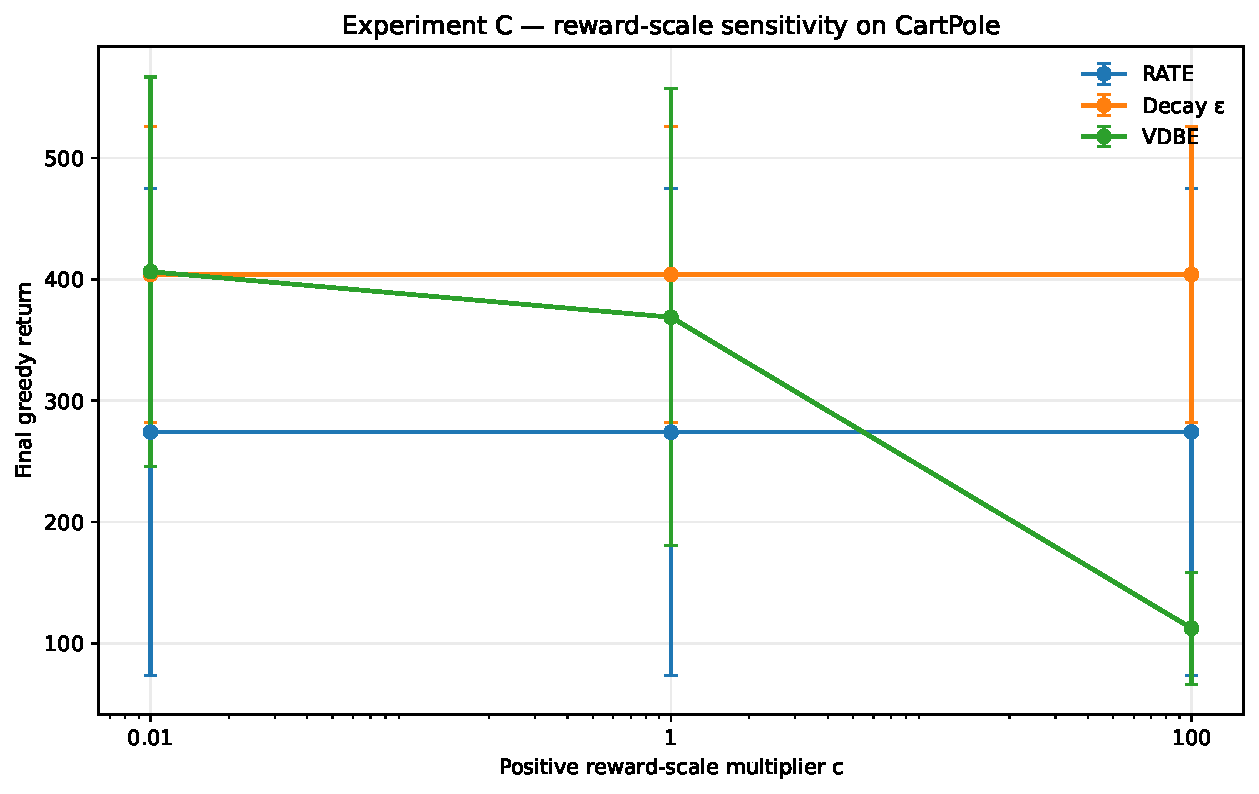
\includegraphics[width=\columnwidth]{src/figures/final/diagnostics/diag_C_reward_scale.pdf}
    \caption{Experiment C: final greedy performance under positive reward rescaling. RATE and the reward-independent decay schedule remain stable, whereas fixed-$\sigma$ VDBE changes substantially.}
    \label{fig:reward-scale}
\end{figure}


\subsection{Fidelity of VDBE Adaptations Under Function Approximation}

The project implementation uses a global VDBE exploration state as a pragmatic adaptation to function approximation. To determine whether its behavior is primarily caused by the choice of TD signal or by the loss of literal state-local exploration memory, we compare four variants: global versus state-local exploration state, each driven by either raw TD error or the corresponding change in action value.

Figure~\ref{fig:vdbe-fidelity} shows little practical difference between the two global-signal variants on MountainCar and Acrobot. In contrast, state-local variants perform substantially worse on Acrobot and maintain very large collections of state-dependent exploration values. This indicates that the principal fidelity-sensitive design choice in this setting is the move from global to literal state-local exploration adaptation, rather than substituting $\Delta Q$ for the raw TD signal alone.

This ablation should not be interpreted as an exact replication of the original tabular VDBE algorithm. The state-local tiled implementation is closer to the original state-specific concept but still operates through function-approximation features rather than a tabular state representation.

\begin{figure}[t]
    \centering
    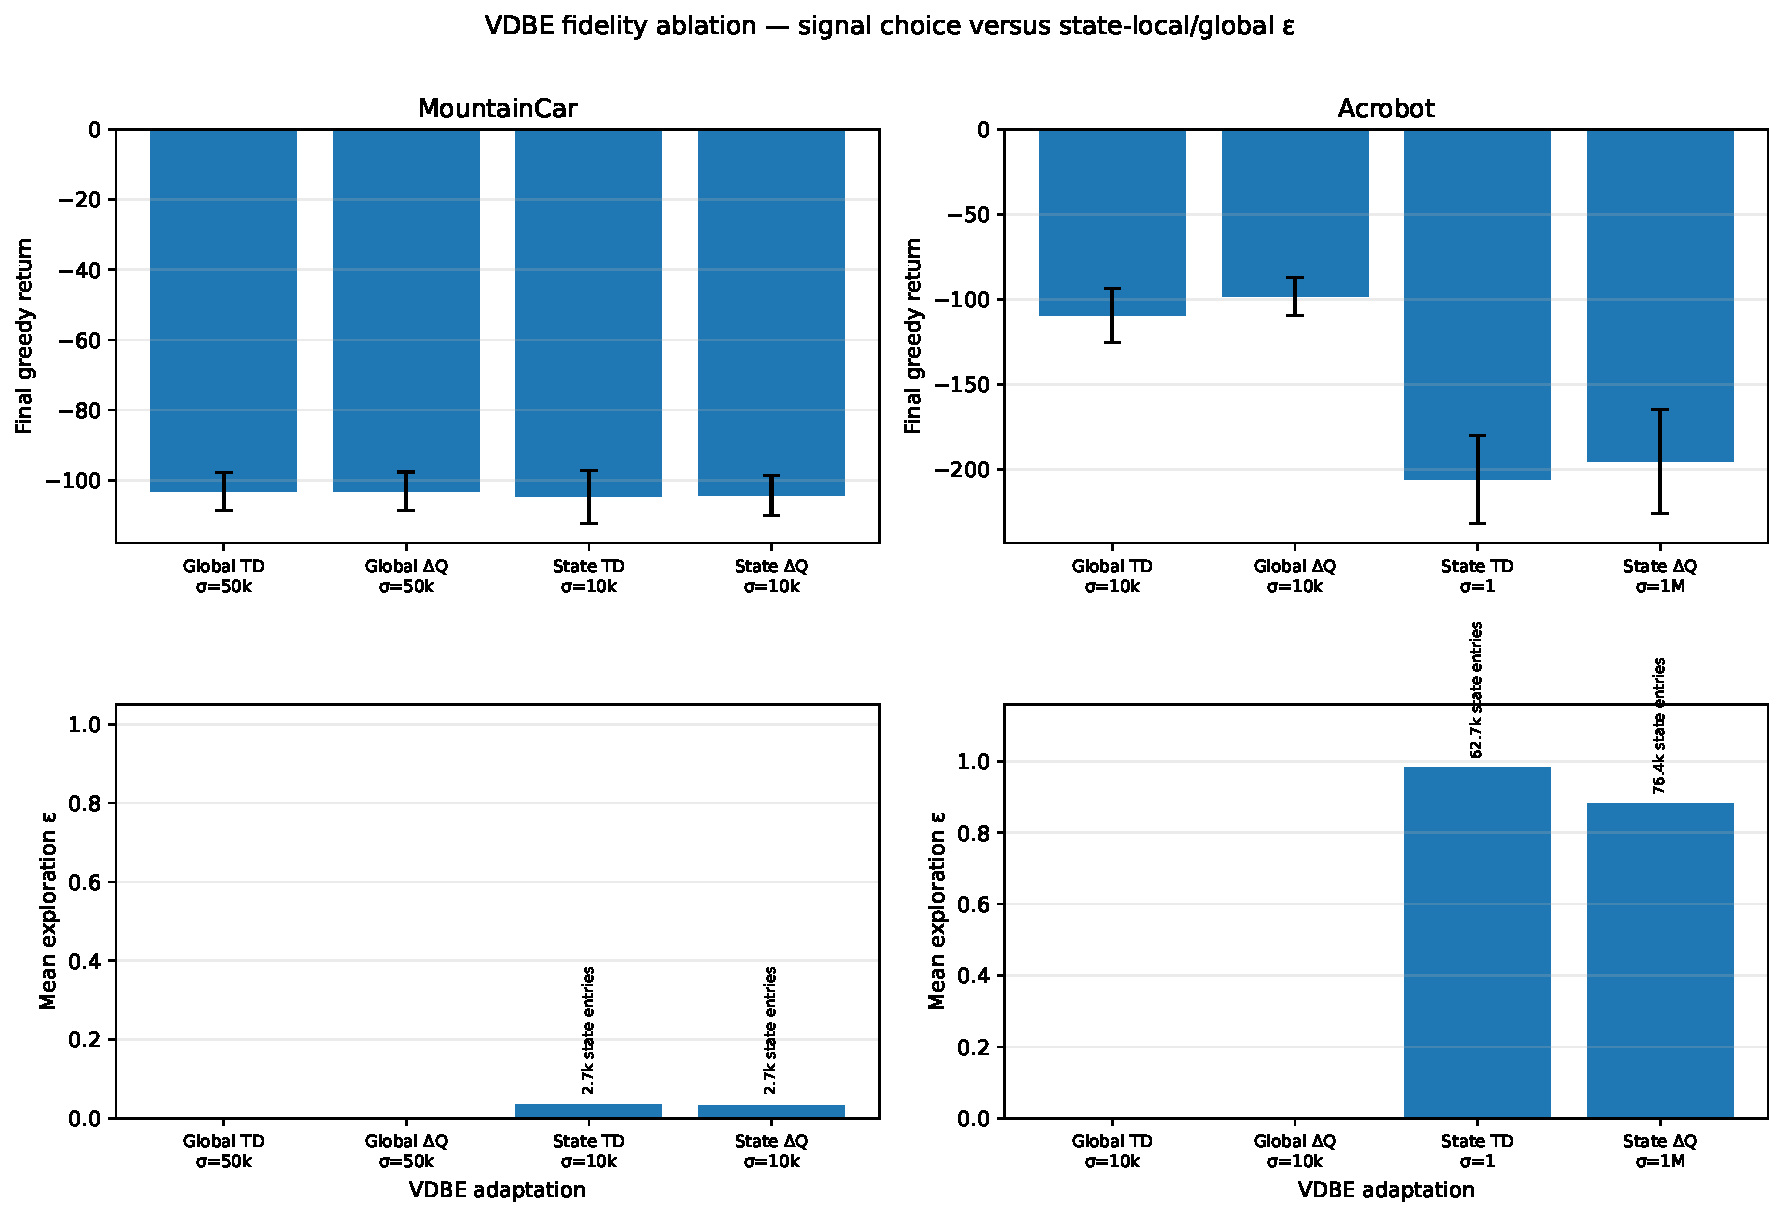
\includegraphics[width=\columnwidth]{src/figures/final/diagnostics/diag_vdbe_fidelity.pdf}
    \caption{VDBE fidelity ablation comparing global and state-local exploration adaptation with TD-error and $\Delta Q$ signals.}
    \label{fig:vdbe-fidelity}
\end{figure}


\subsection{Final Benchmark Under Linear Function Approximation}

We next compare RATE with fixed $\epsilon$-greedy, linear $\epsilon$ decay, Boltzmann exploration, and VDBE using the frozen 30-seed headline protocol. Aggregate performance is computed from normalized final greedy scores using the interquartile mean and stratified bootstrap confidence intervals.

Under linear Sarsa($\lambda$), RATE obtains an aggregate normalized IQM of \LinearRateAggIQM\ with a 95\% bootstrap interval of [\LinearRateAggCILow, \LinearRateAggCIHigh] and ranks \LinearRateRank th among the five methods. RATE strongly improves over fixed $\epsilon$, but does not dominate the tuned adaptive and scheduled baselines. In particular, RATE minus Boltzmann is \LinearRateMinusBoltzmann\ with a 95\% bootstrap interval of [\LinearRateMinusBoltzmannCILow, \LinearRateMinusBoltzmannCIHigh], establishing an aggregate advantage for Boltzmann under this approximator.

Thus, reward-scale robustness does not by itself imply superior exploration performance. The normalization used by RATE removes an undesirable dependence on arbitrary reward magnitude, but it can also produce exploration behavior that is less well matched to a particular approximation regime or task.


\subsection{Final Benchmark Under Double DQN}

The ordering changes substantially under Double DQN. RATE achieves an aggregate normalized IQM of \DQNRateAggIQM\ with a 95\% bootstrap interval of [\DQNRateAggCILow, \DQNRateAggCIHigh] and ranks \DQNRateRank st overall.

RATE minus decay is \DQNRateMinusDecay\ with a 95\% bootstrap interval of [\DQNRateMinusDecayCILow, \DQNRateMinusDecayCIHigh], while RATE minus Boltzmann is \DQNRateMinusBoltzmann\ with interval [\DQNRateMinusBoltzmannCILow, \DQNRateMinusBoltzmannCIHigh]. Both intervals exclude zero. By contrast, the aggregate differences from fixed $\epsilon$ and VDBE remain inconclusive under the corresponding bootstrap intervals.

These aggregate results should be interpreted together with the environment-level results. Double-DQN MountainCar remains close to the failure floor for all five exploration methods. Consequently, statistically detectable differences on that task need not correspond to a practically large improvement in control performance.

\begin{figure}[t]
    \centering
    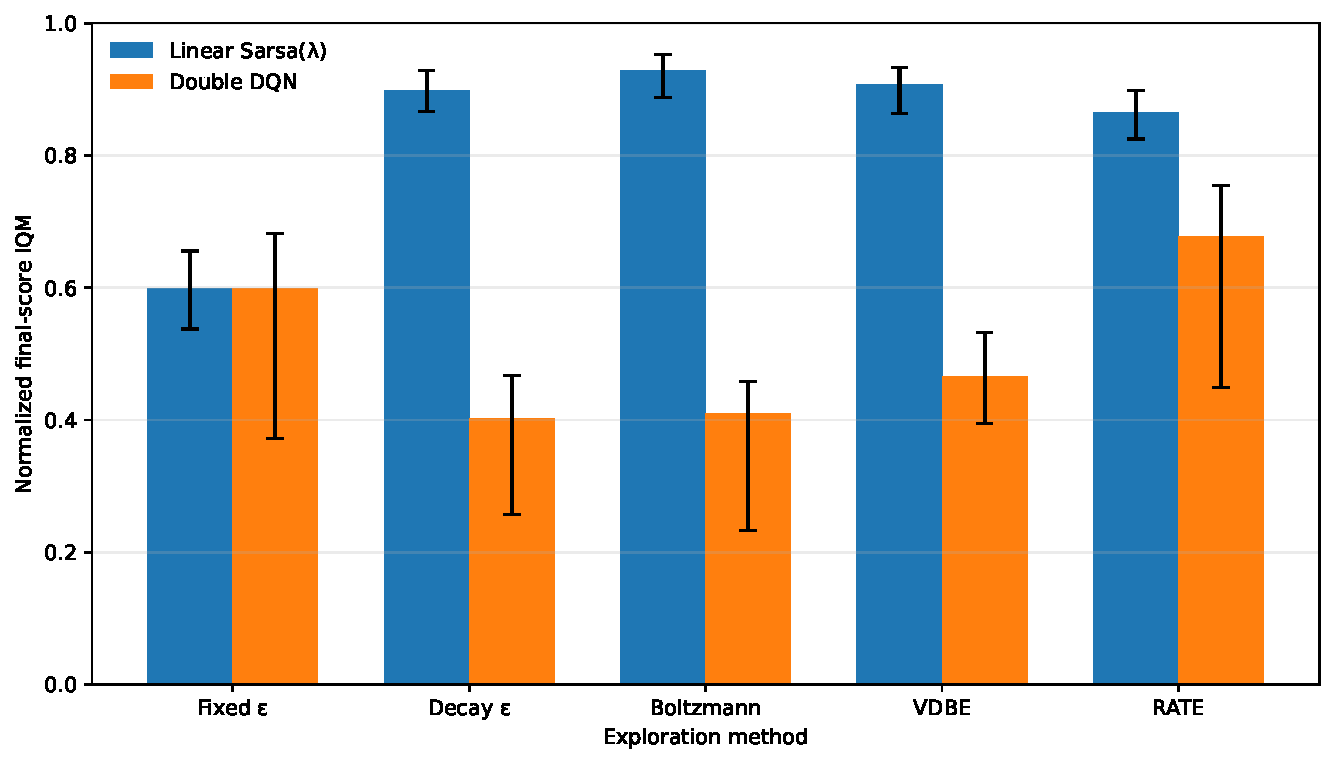
\includegraphics[width=\columnwidth]{src/figures/final/headline_aggregate_iqm.pdf}
    \caption{Aggregate normalized final-score IQM with 95\% stratified bootstrap confidence intervals under linear Sarsa($\lambda$) and Double DQN.}
    \label{fig:headline-aggregate}
\end{figure}


\subsection{Exploration Rankings Depend on the Function Approximator}

The most important combined result is the reversal in exploration-method ordering across the two approximation regimes. RATE moves from rank \LinearRateRank\ under linear approximation to rank \DQNRateRank\ under Double DQN. Conversely, Boltzmann exploration moves from first under the linear agent to fourth under Double DQN.

Figure~\ref{fig:rank-shift} summarizes these changes. The finding rules out a simple universal ranking of the tested exploration strategies. Instead, the interaction between the exploration mechanism, value representation, and learning dynamics appears to determine which exploration rule is most effective.

The rank change itself is descriptive: we did not pre-specify or perform a direct statistical interaction test comparing rank shifts between approximators. We therefore do not claim that the cross-approximator rank reversal is itself statistically significant. The inferential claims remain the within-approximator bootstrap and corrected pairwise comparisons reported above.

\begin{figure}[t]
    \centering
    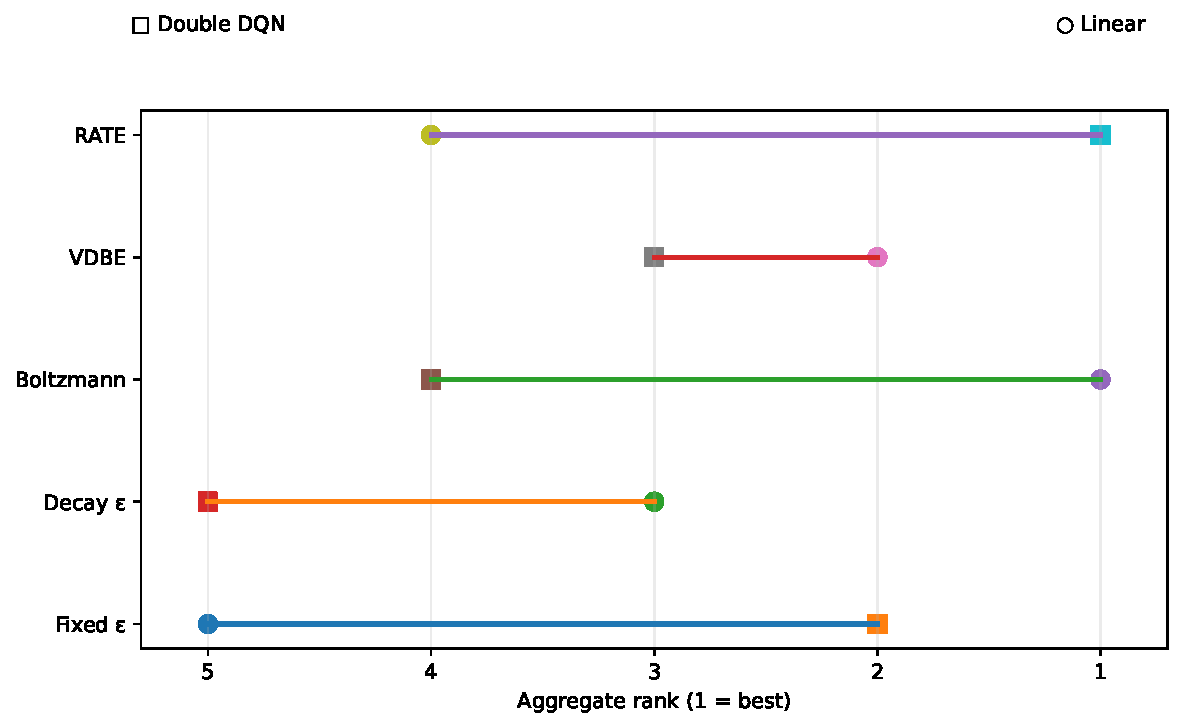
\includegraphics[width=\columnwidth]{src/figures/final/headline_rank_shift.pdf}
    \caption{Descriptive change in aggregate exploration-method ranking between linear Sarsa($\lambda$) and Double DQN.}
    \label{fig:rank-shift}
\end{figure}

\begin{figure}[t]
    \centering
    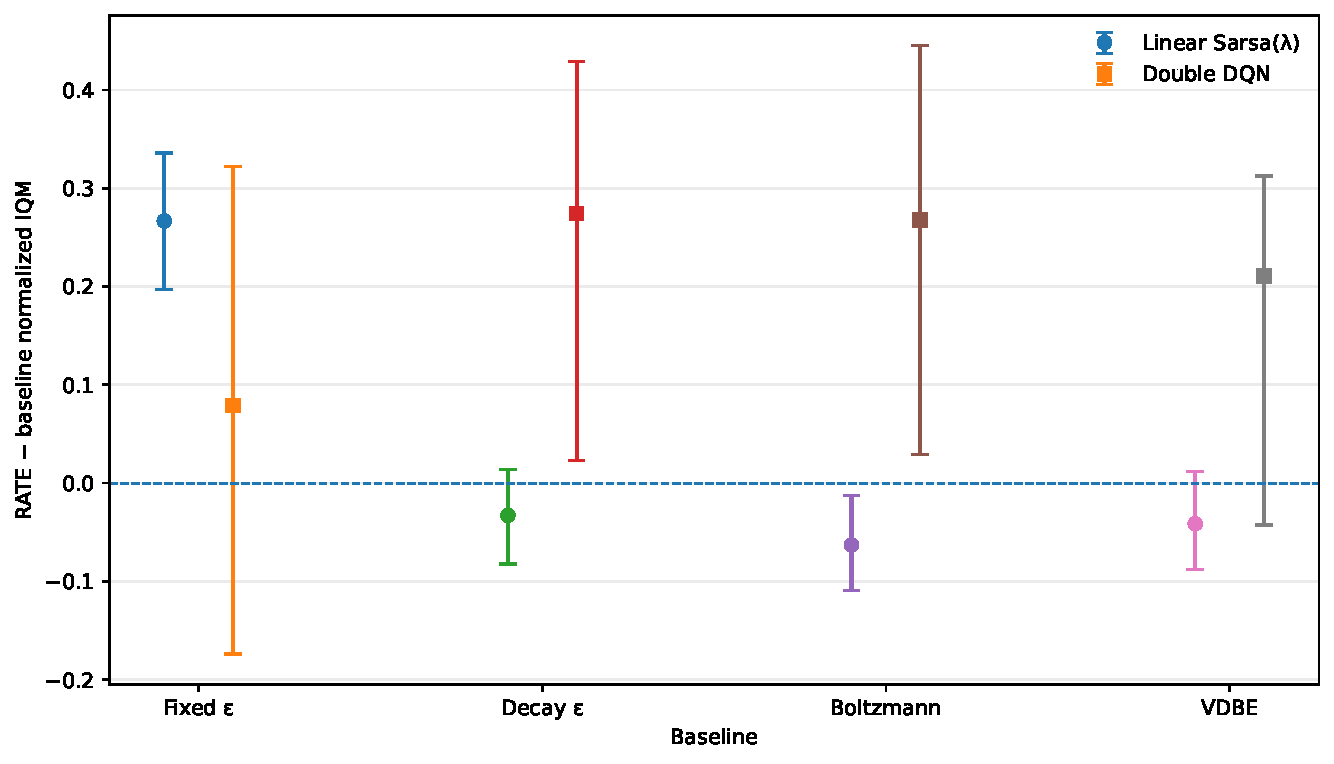
\includegraphics[width=\columnwidth]{src/figures/final/headline_rate_minus_baselines.pdf}
    \caption{Aggregate normalized IQM difference between RATE and each baseline. Positive values favor RATE; intervals are stratified bootstrap confidence intervals.}
    \label{fig:rate-differences}
\end{figure}
